\documentclass[]{article}

\usepackage[italian]{babel}
\usepackage[margin=20mm, footskip = 20pt]{geometry}
\usepackage{array}
\usepackage{tabularx}
\usepackage{graphicx}
\usepackage{subfiles}
\usepackage{hyperref}
\usepackage{nameref}
\usepackage{titlesec}
\usepackage{longtable}
\usepackage[table]{xcolor}
\usepackage{titling}
\usepackage{lastpage}
\usepackage{ifthen}
\usepackage{calc}
\usepackage{soulutf8}
\usepackage{contour}
\usepackage{float}
\usepackage{fancyhdr}
\usepackage{multirow}
\usepackage{pgfgantt}
\usepackage{lscape}

\newcommand{\hr}{\par\vspace{-.1\ht\strutbox}\noindent\hrulefill\par}

\graphicspath{ {./}
	{./commons/res}
}

%--------------------------------------------------
% Comandi per inserire contenuto del documento
%--------------------------------------------------
\makeatletter

\newcommand\appendToGraphicsPath[1]{%
	\g@addto@macro\Ginput@path{{#1}}%
}

\newcommand{\setTitle}[1]{%
	\newcommand{\@phTitle}{#1}%
}
\newcommand{\phTitle}{\@phTitle}

\newcommand{\setDate}[1]{%
	\newcommand{\@phDate}{#1}%
}
\newcommand{\phDate}{\@phDate}

\newcommand{\setUso}[1]{%
	\newcommand{\@uso}{#1}%
}
\newcommand{\uso}{\@uso}

\newcommand{\setVersione}[1]{%
	\newcommand{\@versione}{#1}%
}
\newcommand{\versione}{\@versione}

\newcommand{\disabilitaVersione}{%
	\renewcommand{\setVersione}[1]{}%
	\renewcommand{\versione}{DISABILITATA}
}

\newcommand{\setResponsabile}[1]{%
	\newcommand{\@responsabile}{#1}%
}
\newcommand{\responsabile}{\@responsabile}

\newcommand{\setRedattori}[1]{%
	\newcommand{\@redattori}{#1}%
}
\newcommand{\redattori}{\@redattori}

\newcommand{\setVerificatori}[1]{%
	\newcommand{\@verificatori}{#1}%
}
\newcommand{\verificatori}{\@verificatori}

\newcommand{\setModifiche}[1]{%
	\newcommand{\@modifiche}{#1}%
}
\newcommand{\modifiche}{\@modifiche}

\makeatother 

%--------------------------------------------------
% Comandi per i documenti esterni e il glossario
%--------------------------------------------------

\newcommand{\dext}[1]{\textsc{#1\textsubscript{\textit{D}}}}

\newcommand{\glock}[1]{\textsc{#1\textsubscript{\textit{G}}}}

%--------------------------------------------------
% Comandi per impostare sottotitoli di quarto e quinto livello
%--------------------------------------------------

\setcounter{secnumdepth}{4}
\setcounter{tocdepth}{4}

\titleformat{\paragraph}
{\normalfont\normalsize\bfseries}{\theparagraph}{1em}{}
\titlespacing*{\paragraph}{0pt}{2.25ex plus 1ex minus .2ex}{1.5ex plus .2ex}

\titleformat{\subparagraph}
{\normalfont\normalsize\bfseries}{\thesubparagraph}{1em}{}
\titlespacing*{\subparagraph}{0pt}{1.75ex plus 1ex minus .2ex}{.75ex plus .1ex}

\appendToGraphicsPath{../../../commons/res/}

%------------------------------
%
% COMANDI DI CONFIGURAZIONE
%
%------------------------------

\setTitle{Verbale riunione \#8}

\setVersione{1.0.0}

\setDate{05-12-2020}

\setResponsabile{Alessandro Chimetto}

\setRedattori{Alessandro Chimetto}

\setVerificatori{Valton Tahiraj}

\setUso{Interno}

\setModifiche{
	1.0.0 & Alessandro Chimetto & Responsabile & 9-01-2020 & Approvazione documento\\
	0.1.0 & Valton Tahiraj & Verificatore & 12-12-2020 & Verifica documento\\
	0.0.1 & Alessandro Chimetto & Redattore & 05-12-2020 & Stesura iniziale}

\begin{document}

	% Direttive per la creazione del titolo tramite comando maketitle
\title{\huge \textsc{\phTitle{}} \\
	\vspace{11pt} \large \textsc{\phDate{}}}

\author{} % Non toccare
\date{} % Non toccare

%--------------------
% Frontespizio
%--------------------

% Logo del gruppo
\begin{figure}[t!]
	\centering
	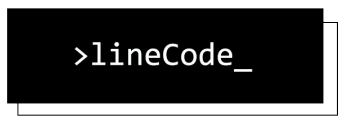
\includegraphics[width=20em]{lclong}
\end{figure}

% Titolo / Nome
\maketitle
\thispagestyle{empty}

% Dati specifici sul doc in forma tabulare
\begin{table}[ht]
	\begin{center}
		\label{tab:Dati sul documento}
		\begin{tabular}{r|l}
			\multicolumn{2}{c}{ \textsc{Dati sul documento} } \\
			\hline
			\textbf{Versione} & \versione{} \\
			\textbf{Uso} & \uso{}  \\
			\textbf{Redattori} & \redattori{} \\
			\textbf{Verificatori} & \verificatori{} \\
			\textbf{Responsabile} & \responsabile{} \\
			\textbf{Destinatari} & lineCode \\
								& prof.\ Vardanega Tullio \\		
								& prof.\ Cardin Riccardo \\
			\ifthenelse{\equal{\uso}{Esterno}}{
								& Sanmarco Informatica
			}{} \\
		\end{tabular}
	\end{center}
\end{table}

\newpage

\renewcommand{\arraystretch}{2} % allarga le righe con dello spazio sotto e sopra
\begin{longtable}[H]{>{\centering\bfseries}m{2cm} >{\centering}m{3.5cm} >{\centering}m{2.5cm} >{\centering}m{3cm} >{\centering\arraybackslash}m{5cm}}
	\rowcolor{lightgray}
	{\textbf{Versione}} & {\textbf{Nominativo}} & {\textbf{Ruolo}} & {\textbf{Data}} & {\textbf{Descrizione}}  \\
	\endfirsthead%
	\rowcolor{lightgray}
	{\textbf{Versione}} & {\textbf{Nominativo}}  & {\textbf{Ruolo}} & {\textbf{Data}} & {\textbf{Descrizione}}  \\
	\endhead%
	\modifiche{}%
\end{longtable}

	\newpage

	%--------------------------------
	%
	% IL CONTENUTO INIZIA DA QUI
	%
	%--------------------------------

	\section{Introduzione}
		\subsection{Luogo e data dell'incontro}
		\begin{itemize}
			\item \textbf{Modalità}: Telematica;
			\item \textbf{Software utilizzato}: \glock{Discord};
			\item \textbf{Data}: 31 Ottobre 2020;
			\item \textbf{Ora di inizio}: 16:00;
			\item \textbf{Ora di fine}: 17:00.
		\end{itemize}

		\subsection{Presenze}
		\begin{itemize}
			\item \textbf{Presenti}:
			\begin{itemize}
				\item Matteo Alba
				\item Giacomo Bulbarelli
				\item Alessandro Chimetto
				\item Alessandro Dindinelli
				\item Lucia Fenu
				\item Paolo Scanferlato
				\item Valton Tahiraj 
			\end{itemize}
			\item \textbf{Assenti}:
			\begin{itemize}
				\item Nessuno
			\end{itemize}
		\end{itemize}


		\subsection{Ordine del giorno}
		\begin{enumerate}
			\item Impressioni su seminari tecnologici appena svolti;
			\item scelta definitiva delle preferenze \glock{capitolati};
			\item discussione sui prossimi passi per la stesura di documentazione;
			\item fissare data e ora per l'incontro successivo;
			\item varie ed eventuali.
		\end{enumerate}

	\newpage

	\section{Svolgimento}
		\subsection{Impressioni su seminari tecnologici}
		Si è discusso dei seminari tecnologici riguardanti i \glock{capitolati} C5 e C6 del giorno 04-12.\\

		\subsection{Scelta definitiva capitolati}
		Essendosi conclusi tutti i seminari tecnologici previsti e avendo fatto il punto della situazione, si è deciso in modo definitivo sui tre \glock{capitolati} più d'interesse per il gruppo ovvero in ordine decrescente: C5, C3, C1.\\

		\subsection{Prossimi passi per stesura documentazione}
		Si è deciso che per le seguenti date saranno pronti in \LaTeX\ i rispettivi documenti che al momento sono delle bozze:
		\begin{itemize}
			\item 13-12 \dext{Studio di Fattibilità v1.0.0};
			\item 20-12 \dext{Norme di Progetto v1.0.0};
			\item 27-12 \dext{Piano di Progetto v1.0.0};
			\item 04-01 \dext{Analisi dei Requisiti v1.0.0};
			\item 07-01 \dext{Piano di Qualifica v1.0.0}.\\
		\end{itemize}

		\subsection{Scelta strumenti di supporto}
		Si è deciso di:
		\begin{itemize}
			\item scrivere la documentazione in \LaTeX\ per permettere il tracciamento delle modifiche tramite sistemi di versionamento;
			\item utilizzare \glock{TeXstudio} come IDE per la scrittura dei documenti \LaTeX;
			\item utilizzare \glock{git} come software di versionamento con \glock{repository} remota su \glock{GitHub}.
		\end{itemize}

		\subsection{Riunione successiva}
		Sono state fissate due riunioni successive.
		Prima riunione fissata:
		\begin{itemize}
			\item \textbf{Data}: Mercoledì 9 Dicembre;
			\item \textbf{Ora}: 21:00;
			\item \textbf{Modalità}: Telematica: \glock{Discord}.
		\end{itemize}
		Seconda riunione fissata:
		\begin{itemize}
			\item \textbf{Data}: Venerdì 11 Dicembre;
			\item \textbf{Ora}: 21:00;
			\item \textbf{Modalità}: Telematica: \glock{Discord}.
		\end{itemize}

\end{document}

